Hier werden die Regressionsnetze mit Early Stopping verwendet und auch erklärt, warum das bei Klassifikation sinnlos ist. 
Dabei werden nur die Direct Cascade Netze betrachtet. 

Sowohl für die Regressionsnetze als auch für die Klassifikationsnetze wurde LM verwendet. 
Zudem für Regression noch MAEM und für Klassifikation ACCM. 

Bei der Klassifikation kommt es nur manchmal zu einem Abbruch der Epochen über das ACCM, aber es wird dadurch nicht besser. Mit LM kommt 
dieser Abbruch öfter vor und das Training geht somit 
zwar schneller, jedoch bleibt Klassifikation mit Kaskadierung so schlecht, dass es nicht genutzt werden kann. Dass weder LM noch ACCM 
funktioniert sieht man deutlich in Figure 5.7. ACCM ist die einzige der hier vorkommenden Metriken, dessen Ziel ein Maximum ist. 

\begin{figure}[htpb]
    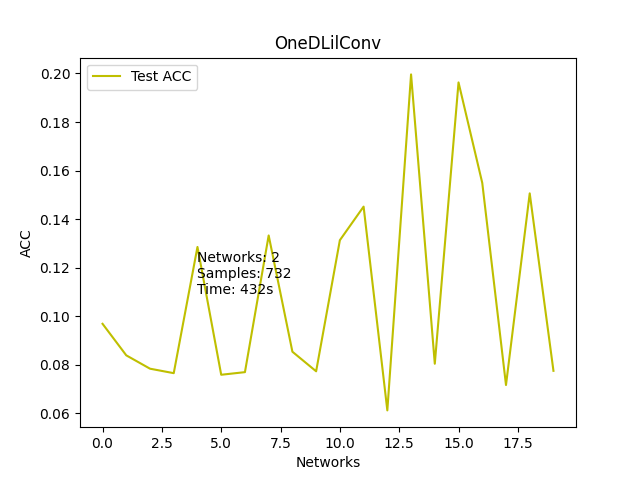
\includegraphics[height=4.5cm]{../../Plots/ba_plots/earlystopping/lossmetric/1dconv_ts.png}
    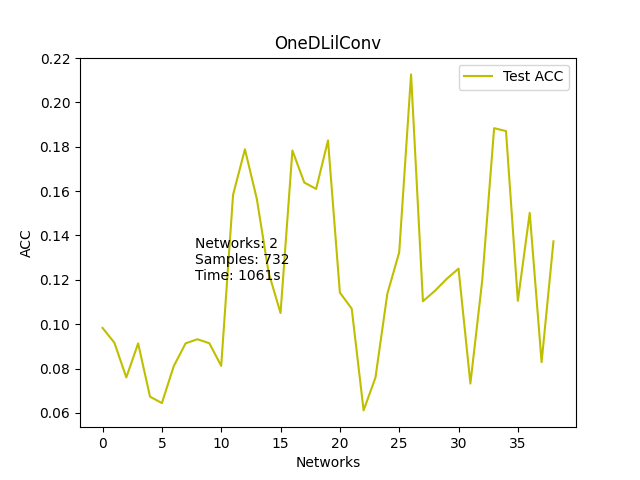
\includegraphics[height=4.5cm]{../../Plots/ba_plots/earlystopping/intermetric/1dconv_ts.png}
    \caption{\label{fig:1dconvmetrics} LM und ACCM mit 1DConv}
\end{figure}

Deshalb wird sich hier eingehender mit dem Regressionsnetz OneLayer befasst. Die Metriken LM und MAEM suchen dabei ein Minimum. 

\begin{figure}[htpb]
    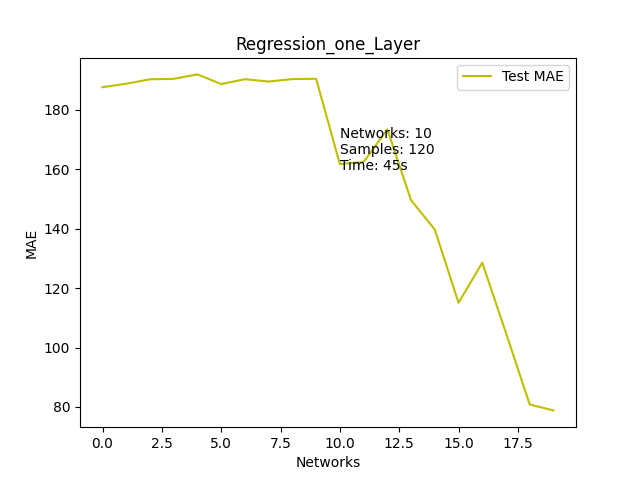
\includegraphics[height=4.5cm]{../../Plots/ba_plots/earlystopping/lossmetric/onelayer_ts.png}
    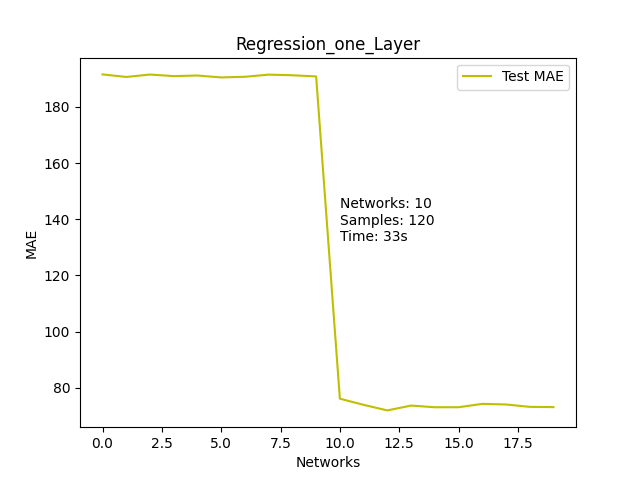
\includegraphics[height=4.5cm]{../../Plots/ba_plots/earlystopping/intermetric/onelayer_ts.png}
    \caption{\label{fig:onelayermetrics} LM und MAEM mit OneLayer}
\end{figure}

Dieses liefert mit den beiden Early-Stopping Metriken LM und MAEM 
halbwegs brauchbare Ergebnisse, jedoch sind diese deutlich schlechter als ein Training ohne diese, wie an den Werten von Figure 5.8 abgelesen 
werden kann. 

Diese Werte sind so schlecht als hätte man das OneLayer Netzwerk mit wenigen Targetdaten direkt auf diesen Datensatz lernen lassen. 
Das diese Early-Stopping Metriken so schleht sind, liegt daran, dass sie keine Verschlechterung im Validationset des Datensatzes dulden und ab 
der ersten das Netz der aktuellen Netziteration beenden. Dadurch ist selten das tatsächliche Minimum das, was über den Augmented Vector 
weitergegeben wird, sondern nur ein leicht abweichendes. Dazu kommt, dass diese Metriken nicht das globale Minimum finden können, wenn sie 
auf ein lokales treffen, denn sie werden Versuchen in diesem zu verbleiben. 
